
%% bare_conf.tex
%% V1.4b
%% 2015/08/26
%% by Michael Shell
%% See:
%% http://www.michaelshell.org/
%% for current contact information.
%%
%% This is a skeleton file demonstrating the use of IEEEtran.cls
%% (requires IEEEtran.cls version 1.8b or later) with an IEEE
%% conference paper.
%%
%% Support sites:
%% http://www.michaelshell.org/tex/ieeetran/
%% http://www.ctan.org/pkg/ieeetran
%% and
%% http://www.ieee.org/

%%*************************************************************************
%% Legal Notice:
%% This code is offered as-is without any warranty either expressed or
%% implied; without even the implied warranty of MERCHANTABILITY or
%% FITNESS FOR A PARTICULAR PURPOSE! 
%% User assumes all risk.
%% In no event shall the IEEE or any contributor to this code be liable for
%% any damages or losses, including, but not limited to, incidental,
%% consequential, or any other damages, resulting from the use or misuse
%% of any information contained here.
%%
%% All comments are the opinions of their respective authors and are not
%% necessarily endorsed by the IEEE.
%%
%% This work is distributed under the LaTeX Project Public License (LPPL)
%% ( http://www.latex-project.org/ ) version 1.3, and may be freely used,
%% distributed and modified. A copy of the LPPL, version 1.3, is included
%% in the base LaTeX documentation of all distributions of LaTeX released
%% 2003/12/01 or later.
%% Retain all contribution notices and credits.
%% ** Modified files should be clearly indicated as such, including  **
%% ** renaming them and changing author support contact information. **
%%*************************************************************************


% *** Authors should verify (and, if needed, correct) their LaTeX system  ***
% *** with the testflow diagnostic prior to trusting their LaTeX platform ***
% *** with production work. The IEEE's font choices and paper sizes can   ***
% *** trigger bugs that do not appear when using other class files.       ***                          ***
% The testflow support page is at:
% http://www.michaelshell.org/tex/testflow/



\documentclass[conference]{IEEEtran}
% Some Computer Society conferences also require the compsoc mode option,
% but others use the standard conference format.
%
% If IEEEtran.cls has not been installed into the LaTeX system files,
% manually specify the path to it like:
% \documentclass[conference]{../sty/IEEEtran}





% Some very useful LaTeX packages include:
% (uncomment the ones you want to load)


% *** MISC UTILITY PACKAGES ***
%
%\usepackage{ifpdf}
% Heiko Oberdiek's ifpdf.sty is very useful if you need conditional
% compilation based on whether the output is pdf or dvi.
% usage:
% \ifpdf
%   % pdf code
% \else
%   % dvi code
% \fi
% The latest version of ifpdf.sty can be obtained from:
% http://www.ctan.org/pkg/ifpdf
% Also, note that IEEEtran.cls V1.7 and later provides a builtin
% \ifCLASSINFOpdf conditional that works the same way.
% When switching from latex to pdflatex and vice-versa, the compiler may
% have to be run twice to clear warning/error messages.






% *** CITATION PACKAGES ***
%
%\usepackage{cite}
% cite.sty was written by Donald Arseneau
% V1.6 and later of IEEEtran pre-defines the format of the cite.sty package
% \cite{} output to follow that of the IEEE. Loading the cite package will
% result in citation numbers being automatically sorted and properly
% "compressed/ranged". e.g., [1], [9], [2], [7], [5], [6] without using
% cite.sty will become [1], [2], [5]--[7], [9] using cite.sty. cite.sty's
% \cite will automatically add leading space, if needed. Use cite.sty's
% noadjust option (cite.sty V3.8 and later) if you want to turn this off
% such as if a citation ever needs to be enclosed in parenthesis.
% cite.sty is already installed on most LaTeX systems. Be sure and use
% version 5.0 (2009-03-20) and later if using hyperref.sty.
% The latest version can be obtained at:
% http://www.ctan.org/pkg/cite
% The documentation is contained in the cite.sty file itself.






% *** GRAPHICS RELATED PACKAGES ***
%
\ifCLASSINFOpdf
  % \usepackage[pdftex]{graphicx}
  % declare the path(s) where your graphic files are
  % \graphicspath{{../pdf/}{../jpeg/}}
  % and their extensions so you won't have to specify these with
  % every instance of \includegraphics
  % \DeclareGraphicsExtensions{.pdf,.jpeg,.png}
\else
  % or other class option (dvipsone, dvipdf, if not using dvips). graphicx
  % will default to the driver specified in the system graphics.cfg if no
  % driver is specified.
  % \usepackage[dvips]{graphicx}
  % declare the path(s) where your graphic files are
  % \graphicspath{{../eps/}}
  % and their extensions so you won't have to specify these with
  % every instance of \includegraphics
  % \DeclareGraphicsExtensions{.eps}
\fi
% graphicx was written by David Carlisle and Sebastian Rahtz. It is
% required if you want graphics, photos, etc. graphicx.sty is already
% installed on most LaTeX systems. The latest version and documentation
% can be obtained at: 
% http://www.ctan.org/pkg/graphicx
% Another good source of documentation is "Using Imported Graphics in
% LaTeX2e" by Keith Reckdahl which can be found at:
% http://www.ctan.org/pkg/epslatex
%
% latex, and pdflatex in dvi mode, support graphics in encapsulated
% postscript (.eps) format. pdflatex in pdf mode supports graphics
% in .pdf, .jpeg, .png and .mps (metapost) formats. Users should ensure
% that all non-photo figures use a vector format (.eps, .pdf, .mps) and
% not a bitmapped formats (.jpeg, .png). The IEEE frowns on bitmapped formats
% which can result in "jaggedy"/blurry rendering of lines and letters as
% well as large increases in file sizes.
%
% You can find documentation about the pdfTeX application at:
% http://www.tug.org/applications/pdftex





% *** MATH PACKAGES ***
%
%\usepackage{amsmath}
% A popular package from the American Mathematical Society that provides
% many useful and powerful commands for dealing with mathematics.
%
% Note that the amsmath package sets \interdisplaylinepenalty to 10000
% thus preventing page breaks from occurring within multiline equations. Use:
%\interdisplaylinepenalty=2500
% after loading amsmath to restore such page breaks as IEEEtran.cls normally
% does. amsmath.sty is already installed on most LaTeX systems. The latest
% version and documentation can be obtained at:
% http://www.ctan.org/pkg/amsmath





% *** SPECIALIZED LIST PACKAGES ***
%
%\usepackage{algorithmic}
% algorithmic.sty was written by Peter Williams and Rogerio Brito.
% This package provides an algorithmic environment fo describing algorithms.
% You can use the algorithmic environment in-text or within a figure
% environment to provide for a floating algorithm. Do NOT use the algorithm
% floating environment provided by algorithm.sty (by the same authors) or
% algorithm2e.sty (by Christophe Fiorio) as the IEEE does not use dedicated
% algorithm float types and packages that provide these will not provide
% correct IEEE style captions. The latest version and documentation of
% algorithmic.sty can be obtained at:
% http://www.ctan.org/pkg/algorithms
% Also of interest may be the (relatively newer and more customizable)
% algorithmicx.sty package by Szasz Janos:
% http://www.ctan.org/pkg/algorithmicx




% *** ALIGNMENT PACKAGES ***
%
%\usepackage{array}
% Frank Mittelbach's and David Carlisle's array.sty patches and improves
% the standard LaTeX2e array and tabular environments to provide better
% appearance and additional user controls. As the default LaTeX2e table
% generation code is lacking to the point of almost being broken with
% respect to the quality of the end results, all users are strongly
% advised to use an enhanced (at the very least that provided by array.sty)
% set of table tools. array.sty is already installed on most systems. The
% latest version and documentation can be obtained at:
% http://www.ctan.org/pkg/array


% IEEEtran contains the IEEEeqnarray family of commands that can be used to
% generate multiline equations as well as matrices, tables, etc., of high
% quality.




% *** SUBFIGURE PACKAGES ***
%\ifCLASSOPTIONcompsoc
%  \usepackage[caption=false,font=normalsize,labelfont=sf,textfont=sf]{subfig}
%\else
%  \usepackage[caption=false,font=footnotesize]{subfig}
%\fi
% subfig.sty, written by Steven Douglas Cochran, is the modern replacement
% for subfigure.sty, the latter of which is no longer maintained and is
% incompatible with some LaTeX packages including fixltx2e. However,
% subfig.sty requires and automatically loads Axel Sommerfeldt's caption.sty
% which will override IEEEtran.cls' handling of captions and this will result
% in non-IEEE style figure/table captions. To prevent this problem, be sure
% and invoke subfig.sty's "caption=false" package option (available since
% subfig.sty version 1.3, 2005/06/28) as this is will preserve IEEEtran.cls
% handling of captions.
% Note that the Computer Society format requires a larger sans serif font
% than the serif footnote size font used in traditional IEEE formatting
% and thus the need to invoke different subfig.sty package options depending
% on whether compsoc mode has been enabled.
%
% The latest version and documentation of subfig.sty can be obtained at:
% http://www.ctan.org/pkg/subfig




% *** FLOAT PACKAGES ***
%
%\usepackage{fixltx2e}
% fixltx2e, the successor to the earlier fix2col.sty, was written by
% Frank Mittelbach and David Carlisle. This package corrects a few problems
% in the LaTeX2e kernel, the most notable of which is that in current
% LaTeX2e releases, the ordering of single and double column floats is not
% guaranteed to be preserved. Thus, an unpatched LaTeX2e can allow a
% single column figure to be placed prior to an earlier double 
% figure.
% Be aware that LaTeX2e kernels dated 2015 and later have fixltx2e.sty's
% corrections already built into the system in which case a warning will
% be issued if an attempt is made to load fixltx2e.sty as it is no longer
% needed.
% The latest version and documentation can be found at:
% http://www.ctan.org/pkg/fixltx2e


%\usepackage{stfloats}
% stfloats.sty was written by Sigitas Tolusis. This package gives LaTeX2e
% the ability to do double column floats at the bottom of the page as well
% as the top. (e.g., "\begin{figure*}[!b]" is not normally possible in
% LaTeX2e). It also provides a command:
%\fnbelowfloat
% to enable the placement of footnotes below bottom floats (the standard
% LaTeX2e kernel puts them above bottom floats). This is an invasive package
% which rewrites many portions of the LaTeX2e float routines. It may not work
% with other packages that modify the LaTeX2e float routines. The latest
% version and documentation can be obtained at:
% http://www.ctan.org/pkg/stfloats
% Do not use the stfloats baselinefloat ability as the IEEE does not allow
% \baselineskip to stretch. Authors submitting work to the IEEE should note
% that the IEEE rarely uses double column equations and that authors should try
% to avoid such use. Do not be tempted to use the cuted.sty or midfloat.sty
% packages (also by Sigitas Tolusis) as the IEEE does not format its papers in
% such ways.
% Do not attempt to use stfloats with fixltx2e as they are incompatible.
% Instead, use Morten Hogholm'a dblfloatfix which combines the features
% of both fixltx2e and stfloats:
%
% \usepackage{dblfloatfix}
% The latest version can be found at:
% http://www.ctan.org/pkg/dblfloatfix




% *** PDF, URL AND HYPERLINK PACKAGES ***
%
%\usepackage{url}
% url.sty was written by Donald Arseneau. It provides better support for
% handling and breaking URLs. url.sty is already installed on most LaTeX
% systems. The latest version and documentation can be obtained at:
% http://www.ctan.org/pkg/url
% Basically, \url{my_url_here}.




% *** Do not adjust lengths that control margins, column widths, etc. ***
% *** Do not use packages that alter fonts (such as pslatex).         ***
% There should be no need to do such things with IEEEtran.cls V1.6 and later.
% (Unless specifically asked to do so by the journal or conference you plan
% to submit to, of course. )

\usepackage{tikz}
\usepackage{pdfpages}
\usepackage{pgfplots}
% correct bad hyphenation here
\hyphenation{op-tical net-works semi-conduc-tor}


\begin{document}
%
% paper title
% Titles are generally capitalized except for words such as a, an, and, as,
% at, but, by, for, in, nor, of, on, or, the, to and up, which are usually
% not capitalized unless they are the first or last word of the title.
% Linebreaks \\ can be used within to get better formatting as desired.
% Do not put math or special symbols in the title.
\title{Artificial Immune based Bot for planetWar game}


% author names and affiliations
% use a multiple column layout for up to three different
% affiliations
\author{\IEEEauthorblockN{Mohamed Amine Chikh Touami\\ and SALEM Mohammed}
\IEEEauthorblockA{Faculty of Exact Sciences,\\
University Mustapha Stembouli\\
Mascara, Algeria\\
Email: ma\_chikhtouhami@hotmail.com}
\and
%\IEEEauthorblockN{SALEM Mohammed}
%\IEEEauthorblockA{Faculty of Exact Sciences,\\
%	University Mustapha Stembouli\\
%	Mascara, Algeria\\
%	Email: salem@univ-mascara.dz}
%\and
\IEEEauthorblockN{KHELFI Mohammed Faycal}
\IEEEauthorblockA{RIIR Lab\\
University of Oran 1, Ahmed Ben Bella, Oran, Algeria\\
Email: mf\_khelfi@yahoo.fr}
}

% conference papers do not typically use \thanks and this command
% is locked out in conference mode. If really needed, such as for
% the acknowledgment of grants, issue a \IEEEoverridecommandlockouts
% after \documentclass

% for over three affiliations, or if they all won't fit within the width
% of the page, use this alternative format:
% 
%\author{\IEEEauthorblockN{Michael Shell\IEEEauthorrefmark{1},
%Homer Simpson\IEEEauthorrefmark{2},
%James Kirk\IEEEauthorrefmark{3}, 
%Montgomery Scott\IEEEauthorrefmark{3} and
%Eldon Tyrell\IEEEauthorrefmark{4}}
%\IEEEauthorblockA{\IEEEauthorrefmark{1}School of Electrical and Computer Engineering\\
%Georgia Institute of Technology,
%Atlanta, Georgia 30332--0250\\ Email: see http://www.michaelshell.org/contact.html}
%\IEEEauthorblockA{\IEEEauthorrefmark{2}Twentieth Century Fox, Springfield, USA\\
%Email: homer@thesimpsons.com}
%\IEEEauthorblockA{\IEEEauthorrefmark{3}Starfleet Academy, San Francisco, California 96678-2391\\
%Telephone: (800) 555--1212, Fax: (888) 555--1212}
%\IEEEauthorblockA{\IEEEauthorrefmark{4}Tyrell Inc., 123 Replicant Street, Los Angeles, California 90210--4321}}




% use for special paper notices
%\IEEEspecialpapernotice{(Invited Paper)}




% make the title area
\maketitle

% As a general rule, do not put math, special symbols or citations
% in the abstract
\begin{abstract}
To evolve a decision engine for an autonomous agent, this paper will represent an Evolutionary Algorithm to define a set of rules that the bot based on to achieve some goals in the game.  Planet war is the game used in this study, which Google AI community has been choosing it as a game for their Google AI challenge in 2010, requires that the bot reach some adaptabilities in the aim of beat different enemies in different kind of maps. The Evolutionary Algorithm used to tune multiple parameters to define the bot's behavior.
\end{abstract}

% no keywords




% For peer review papers, you can put extra information on the cover
% page as needed:
% \ifCLASSOPTIONpeerreview
% \begin{center} \bfseries EDICS Category: 3-BBND \end{center}
% \fi
%
% For peerreview papers, this IEEEtran command inserts a page break and
% creates the second title. It will be ignored for other modes.
\IEEEpeerreviewmaketitle



\section{Introduction}
% no \IEEEPARstart
the large entertainment industry sector is the video games.
the commercial Video games budget is rising every year,
it reaches 25.1 billion dollars in 2010\cite{doc2}. Many designers and developers are interested in the community of video games around the world. The main objective of these video games community is to provide amusement to their players.The question is how to do the this; there has been no detailed investigation of the full mechanism to put the work in the correct way.\cite{doc5}
In the past, a number of researchers have sought to determine more realistic games.the developers overlooked their games artificial intelligence and focusing their works to high-quality graphics games.In the last year, these features are not sufficient to guarantee a good profit to the games companies. Moreover, the human players are able to defeat these games without much effort and lose the interest. In the recent years, there has been an increasing interest about more features in video games community such as art, psychology narrative to name but a few.\cite{doc5}  \\

In light of recent events in video games, it is becoming extremely difficult to ignore the existence of one paradigm that is fast becoming a key instrument in most video games is the Artificial Intelligence. The AI is an important aspect of the conception of this kind of games.Moreover, it has seen the rapid of development in many fields such as human player imitation, procedural content generation(PCG), automating game testing, opponent modeling, and computational narrative, among others.\cite{doc5} Recent development in the AI such as computational intelligence and their applications heightened the need for new challenges to the video games community. Whilst, the debate continues about the best strategies for the management of all these features and technics.\cite{doc5} Nonetheless, in the past, developers focusing their works on non-players-characters (NPCs) games to control and design the behavior of the players by the integration of the AI for the opponent modeling to design an intelligent player behavior, in order to increase the player interest on these games.\cite{doc5} \\

The NPCs developers are conscious that stupid behavior of a virtual player will make this kind of games less interesting and easy to beat. As a solution the video games designers new playing rules such as play around levels.In addition, the difficulties are increased from the bottom levels to the high levels.However, players lose their interesting about these games when they are able to win and defeat all the opponents in the end of the game. Whilst, to make an opponent's behavior evolve with player's abilities is an interesting challenge for developers to make this kind of games more attractive. A considerable amount propositions of literature has been published about behavior's self-adapt to players abilities.\cite{doc5}\\

Recently, researchers have shown an increased interest in developing of AI for RTS games. RTS games are a sub-genre of strategy video games, which all the actions made in real-time. The contenders have the capability to control (make a decision) a set of distributed units and structures during the game with the aim of (a) destroy the opponent assets (b)create additional structures to reached some goals in the game or to secure area.\cite{doc5,doc1,doc2,doc3,doc4} The RTS games can be considered as a resource gathering games. Typically, the participants have the possibility to create more units but it's depending on the number of resource gathering with specific units in a specific zone on the map, in order to achieve multiple objectives during the game.\cite{doc5,doc2} At the most of RTS games they employ two levels of AI\cite{doc1}, while can classify these two levels by (a)strategic when it will make a decision over the whole set of units (b) tactical when they decide the behavior of each these small units.In addition, by the real time aspect challenge these difficulties are increased.One of the greatest challenges inherently bounded to the RTS games is the real-time aspect\cite{doc3}. It associated to make the decision without waiting for the others to move. Moreover, the actions are made simultaneously during the course of the game. Some researchers have been carried out on these challenges on the computational intelligence in the game conference (IEEE CIG 2010) while less than 10\% of them deal with it.\cite{doc1,doc3} One of the international AI challenges is Google AI challenge. Which, the participants with the aim to design an AI programs(bots) to play a real-time strategy game. \\

One of the hardest tasks in RTS games is the bots conception. For simulating the other contenders, designers use the bot concept.Bots are intelligent agents interact with human players in order to compete them within any computer-based framework\cite{doc4}.This challenge is made by experts human to design bots behavior from their life experiences and experimentation in order to increase the game's challenges.\cite{doc3} The intelligence bots have a pivotal role\cite{doc4} in the conception of an RTS games. In addition, a set of parameters are required previous the running of the bot, moreover a good parameters values are make a better behavior from the bot. So, for tuning the parameters previously, is wide research area like an optimization problem itself.\cite{doc1} This technic is used to determine which parameters are more important for the bot to tune.\cite{doc1}In a typical RTS games, the contenders(two players or more) have to make a decision under the uncertainty\cite{doc4}(the map is covering by a fog of war, the player will just know their units and structure in the game). There are more difficulties need to understand\cite{doc4} such as spatial reasoning, strategy planning, and opponent's strategy prediction. Therefore, there are hundreds of units simultaneously acting, many possible positions on the map, units control, among others make the conception of the game more challenging and open a wide space of researches. However, current methods of computational intelligence have proven many types of research proposed potential solutions to solve different tasks such as player experience modeling (PEM), procedural content generation (PCG) and data mining\cite{doc2}.\\

RTS games are essential for the wide range of technologies\cite{doc5} in order to design AI, e.g., planning in the uncertainty(lack of information), opponent modeling, temporal reasoning, just to name a few. Like a classic problem, is to provide a non-cheating and humain-like as an important features in the conception of the virtuel players(bots).         
% You must have at least 2 lines in the paragraph with the drop letter
% (should never be an issue)


%\hfill mds
 
%\hfill August 26, 2015

\section{Planet War}
As we mentioned previously one of the international AI competition is organized by google community. In 2010 google choose like a game planet wars for it AI challenge competition. In this pager, we work with a version of Glacon game in order to design a fighter bots. A planet war match\cite{doc1} runs on a map with several distributed planets in different positions, such as each of them has a number describes the quantity of starships its owns. In each turn, the number of starship will change. Each planet is owned by a player, opponent or neutral planet(owned by nobody), moreover, each planet belongs to the player (no neutral one) will increase their number of starships after each step according to their growth rate, this rate explain the additional starship's number will generate each planet in each step.
The main purpose of the planet war game\cite{doc1} is to challenge all players and try to defeat all of them, that mean to destroy all enemy's starships. Planet war is an RTS game by its nature. to achieve a specific objective each player has a limit number of turns to do it and try to win (beat opponent).  \\

\begin{figure}
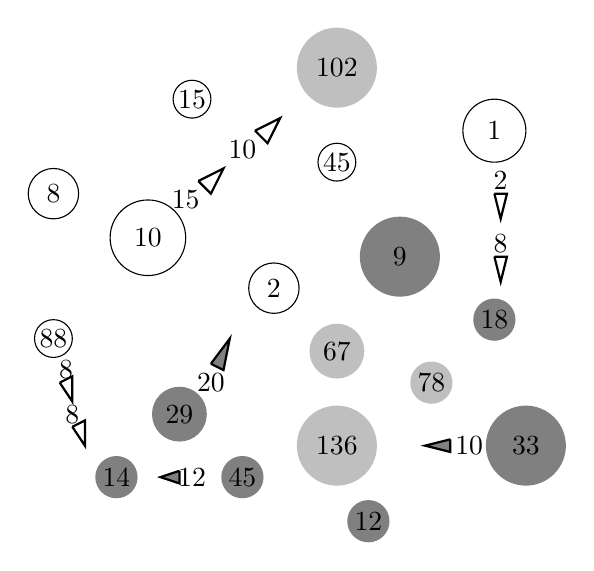
\begin{tikzpicture}[scale = 0.8]
\draw [fill =gray, ultra thick, gray] (2,1) circle [radius=0.3];
\node at (2,1) {14};
\draw [fill =gray, ultra thick, gray] (3,2) circle [radius=0.4];
\draw [fill = gray ,thick] (3.5,2.8) to (3.7,2.7) to (3.8,3.2) to (3.5,2.8);
\node at (3.5,2.5) {20};
\node at (3,2) {29};
\draw [fill =gray, ultra thick, gray] (4,1) circle [radius=0.3];
\node at (4,1) {45};
\draw [fill =gray ,thick] (3,1.1) to (3,0.9) to (2.7,1) to (3,1.1);
\node at (3.2,1) {12};
\draw [fill =gray, ultra thick, gray] (6,0.3) circle [radius=0.3];
\node at (6,0.3) {12};
\draw [fill =gray, ultra thick, gray] (8.5,1.5) circle [radius=0.6];
\node at (8.5,1.5) {33};
\draw [fill = gray ,thick] (7.3,1.6) to (6.9,1.5) to (7.3,1.4) to (7.3,1.6);
\node at (7.6,1.5) {10};
\draw [fill =gray, ultra thick, gray] (8,3.5) circle [radius=0.3];
\node at (8,3.5) {18};
\draw [fill =gray, ultra thick, gray] (6.5,4.5) circle [radius=0.6];
\node at (6.5,4.5) {9};
%\draw [fill =lightgray, ultra thick, lightgray] (3.5,3) circle [radius=0.3];
%\node at (3.5,3) {78};
\draw [fill =lightgray, ultra thick, lightgray] (5.5,1.5) circle [radius=0.6];
\node at (5.5,1.5) {136};
\draw [fill =lightgray, ultra thick, lightgray] (5.5,3) circle [radius=0.4];
\node at (5.5,3) {67};
\draw [fill =lightgray, ultra thick, lightgray] (7,2.5) circle [radius=0.3];
\node at (7,2.5) {78};
\draw [fill =lightgray, ultra thick, lightgray] (5.5,7.5) circle [radius=0.6];
\node at (5.5,7.5) {102};
\draw (1,3.2) circle [radius=0.3];
\node at (1,3.2) {88};
\draw [thick] (1.1,2.5) to (1.3,2.6) to (1.3,2.2) to (1.1,2.5);
\draw [thick] (1.3,1.8) to (1.5,1.9) to (1.5,1.5) to (1.3,1.8);
\node at (1.2,2.7) {8};
\node at (1.3,2) {8};
\draw  (1,5.5) circle [radius=0.4];
\node at (1,5.5) {8};
\draw  (2.5,4.8) circle [radius=0.6];
\node at (2.5,4.8) {10};
\draw  (3.2,7) circle [radius=0.3];
\draw [thick] (3.3,5.7) to (3.7,5.9) to (3.5,5.5) to (3.3,5.7);
\draw [thick] (4.2,6.5) to (4.6,6.7) to (4.4,6.3) to (4.2,6.5);
\node at (3.1,5.4) {15};
\node at (4,6.2) {10};
\node at (3.2,7) {15};
\draw  (4.5,4) circle [radius=0.4];
\node at (4.5,4) {2};
\draw  (5.5,6) circle [radius=0.3];
\node at (5.5,6) {45};
\draw  (8,6.5) circle [radius=0.5];
\draw [thick] (8,5.5) to (8.2,5.5) to (8.1,5.1) to (8,5.5);
\draw [thick] (8,4.5) to (8.2,4.5) to (8.1,4.1) to (8,4.5);
\node at (8,6.5) {1};
\node at (8.1,5.7) {2};
\node at (8.1,4.7) {8};
\end{tikzpicture}
\caption{an early stage of a planet wars game, as shown here there are planet categories, the darker grey (red in the game) ones related to the player, the white ones (green in the game) related to the opponent and the neutral planets are coloured by light grey. Fleets presented by triangles and the numbers are the starships included on them.}
\end{figure}


Moreover, the bot's design faces two major problems: the first one \cite{doc1}is that the bot can't store any information about its previous turns like actions it did, actions of its opponent or even the map's state. Since in each turn, the bot meets with an unknown map as it just begins the game for the first time. The second one\cite{doc3} is that the time requires to move(make an action) is just one second. So these difficulties make the bot's design like a great challenge. In this kind of game, everything has a sum of properties\cite{doc1}. Such as, planets have the x and y coordination for their locations in the map, ownersID, number of starship and growth rate. To conquest other planets, the player needs to send fleets for this aim.Each fleet has a playerID parameter, number of starships, source planetID, destination planetID, turn's number need to reach the target. In each simulated turn\cite{doc1}, the player has the ability to send fleets in a battle with other planet's starships with the source planetID and target planetID, while, the player has the ability\cite{doc1} to make just one action per turn. After each move (action) the planets belong to the players\cite{doc5} increase their ship's number according to their growth rate. To make fleets previously sent reach enemies planets its take time of many turns according to the distance between the source planet and the target planet, moreover, if the source and target planet owned by the same player then it considered like a reinforcment\cite{doc1,doc5} by adding the ship's number on the fleet to the number hosted on the target planet. when the fleets reach the target its will make battles with local target ships, otherwise, if the target is a neutral planet, the player must to sends at least one additional ship to own the planet. While, if the target is owned by the enemy the two players will fight until one with the highest starship number owns the planet. When the player sent fleets to reach some goals\cite{doc5}, he can't change their directions. In addition, the player can send more fleet in the next turns even that the first ones do not yet arrive at their destinations. In the end of the match\cite{doc5}, the player with the highest number of starships wins. If a player loses all their starships then the game will end also faster. whilst, the players have the same starship's number at the end of the game there is a draw\cite{doc5}. 
\section{immune system overview}

One of the most inspirational things that computational based to solve their problems\cite{doc7} is the biology and its various concepts. Among the natural concepts, the immune system has emerged as one of the important aspects to design optimisation algorithms. An optimization problem\cite{doc6} is to look for the optimum element from a set of potential solutions. There are many optimization problems in all of the scientific areas. For this purpose, many methods and algorithms have been developed. The most useful algorithms\cite{doc6} are heuristics.They include divers algorithms such as artificial bee colony, firefly swarm optimisation, ant colony optimization, genetic algorithms, just to mention a few. While the Artificial immune system (AIS) is a common algorithm devised by Decastro\cite{doc6} that uses population-based heuristic concept. The mechanisms used in the biological immune system against various types of pathogens made this system more interesting\cite{doc9} for computer researchers to exploit its technics. This kind of algorithms is used to solve many different optimization problems in science and technology areas. However, the immune system is more complex and its application in technologies areas is a challenge, likewise, the biological immune system\cite{doc7} still under wide active research, whilst, the AIS is adopted just for few mechanisms inspired from the human immune system including the clonal selection.
\subsection{natural immune system}
The biological immune system including human system contains cells, molecules, and organs in its structure to defend the body against the diseases. In the aim to make an immune response\cite{doc6}, the system has to distinguish between the body cells as a self-cells and the foreign cells as nonself-cells(antigens). The immune system response is activated by a suitable mechanism\cite{doc6} to defeat the nonself-cells, this mechanism is defined by the type of the antigens, specific antigen implies a specific response and a specific process. In order to make a fast response in case of the similar antigen, the immune system develops memory cells for this purpose.
\subsubsection*{Clonal selection}
One of the important mechanism used to defend against the nonself-cells\cite{doc6} is the clonal selection. This immune response describes the process how the immune system will stimulus against a specific antigen\cite{doc7} by proliferating a specific type of cells that only those can recognize the antigen.\\
When the antigen is inside the body, the immune response\cite{doc6} by giving the B-cells the ability to secrete antibodies. After that, the T-cells give a signal to the B-cells to proliferate and mature to terminal antibodies secreting cells, it's the plasma cells. The proliferation of the B-cells is according to the affinity level, higher affinity implies more clone will be generated, this whole process named affinity maturation.

\begin{figure}
\begin{tabular}{c}
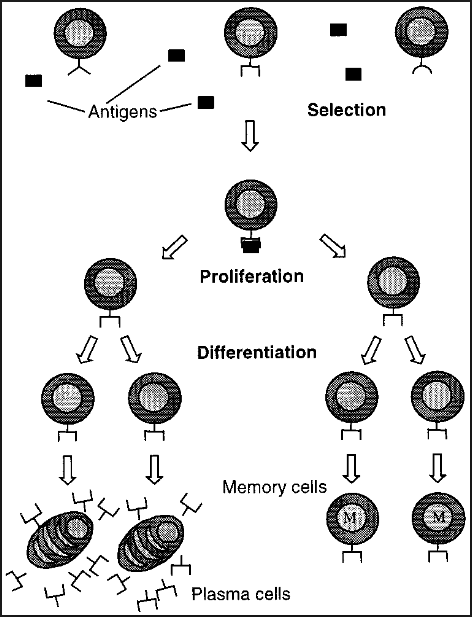
\includegraphics[scale = 0.8]{clonaS}
\end{tabular}
\caption{The biological clonal selection mechanism and its steps in order to defend the body, starting by detecting of the antigen until removing it.}
\end{figure}

The clonal selection process will pass with various steps\cite{doc7}:
\paragraph{•}
The cloned cells undergo to a mutation process.
\paragraph{•}
the self-reactive receptor will be eliminated.
\paragraph{•}
proliferate the mature cells those can detect the antigen.

\subsection{Artificial Immune System}
Inspiring from the biological immune system an algorithm has been developed called Artificial Immune System (AIS)\cite{doc6}. The search technic is similar to the natural immune system by the implication between the fitness function and the affinity maturation in the natural system.
\subsubsection{Initialisation}
A random population N is generated in the search space, as a process that used in the other heuristic algorithms. This population considered like antibodies.
\subsubsection{Clonal proliferation}
In this step, the antibodies will clone (proliferate) according to their fitness(affinity).
\subsubsection{Maturation}
The maturation technic is similar to the mutation one with a mutation probability P. this mutation is applied to equation (1) : 
\begin{equation}
x_{id} = x_{id} + k(x_{d_{max}} - x_{d_{min}}) . N(0,1)
\end{equation}
where $x_{id}$ represent the dimension d of the antibody i, $x_{max}$ and $x_{min}$ represent the min and the max bounds of the variable i, N(0,1) is the standard distribution and k is the scale factor.
\subsubsection{Evaluation}
In the evaluation step, the fitness function of every antibody is calculated by computing the affinity values.
\subsubsection{Ageing operator}
This factor is used to eliminate the individuals lost more. Indeed, the Ageing operator leads to upgrading the initial population.
\subsubsection{Selection process}
This section will be applied to select N individual to the next generation. 
%\subsection{AIS pseudocode}
%\begin{enumerate}
%\item initialize N individual with random values between 0 and 1.
%\item For iteration = 1 : maxIteration,
%\begin{itemize}
%\item Compute the affinities.
%\item Clone the antibodies.
%\item Mutate the antibodies cloned in the previous step.
%\item Compute the affinities for the new antibodies mutated.
%\item Applied the selection process to select the next generation
%\end{itemize} 
%End For \\
%Display the optimal solutions. \\
%End
%\end{enumerate}
\begin{figure}
\centering
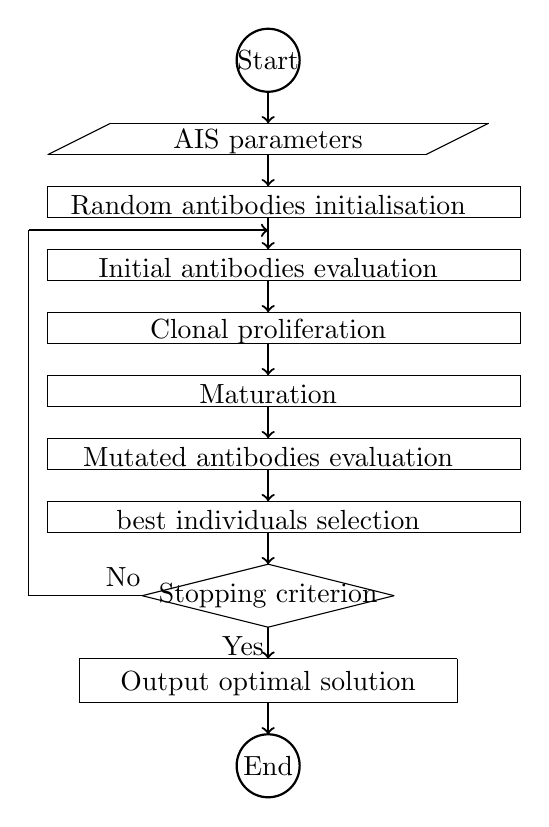
\begin{tikzpicture}[scale = 0.8]
\draw [thick] (4.5,20) circle [radius=0.5];
\node at (4.5,20) {Start};
\draw [->] [thick](4.5,19.5) -- (4.5,19);
\draw (2,19) --(8,19);
\draw (1,18.5) --(7,18.5);
\draw (2,19) --(1,18.5);
\draw (8,19) --(7,18.5);
\node at (4.5,18.7) {AIS parameters};
\draw [->] [thick](4.5,18.5) -- (4.5,18);
\draw (1,18) --(8.5,18);
\draw (1,17.5) --(8.5,17.5);
\draw (1,18) --(1,17.5);
\draw (8.5,18) --(8.5,17.5);
\node at (4.5,17.7) {Random antibodies initialisation};
\draw [->] [thick](4.5,17.5) -- (4.5,17);
\draw (1,17) --(8.5,17);
\draw (1,16.5) --(8.5,16.5);
\draw (1,17) --(1,16.5);
\draw (8.5,17) --(8.5,16.5);
\node at (4.5,16.7) {Initial antibodies evaluation};
\draw [->] [thick](4.5,16.5) -- (4.5,16);
\draw (1,16) --(8.5,16);
\draw (1,15.5) --(8.5,15.5);
\draw (1,15.5) --(1,16);
\draw (8.5,15.5) --(8.5,16);
\node at (4.5,15.7) {Clonal proliferation};
\draw [->][thick] (4.5,15.5) -- (4.5,15);
\draw (1,15) --(8.5,15);
\draw (1,14.5) --(8.5,14.5);
\draw (1,14.5) --(1,15);
\draw (8.5,14.5) --(8.5,15);
\node at (4.5,14.7) {Maturation};
\draw [->][thick] (4.5,14.5) -- (4.5,14);
\draw (1,14) --(8.5,14);
\draw (1,13.5) --(8.5,13.5);
\draw (1,13.5) --(1,14);
\draw (8.5,13.5) --(8.5,14);
\node at (4.5,13.7) {Mutated antibodies evaluation};
\draw [->][thick] (4.5,13.5) -- (4.5,13);
\draw (1,13) --(8.5,13);
\draw (1,12.5) --(8.5,12.5);
\draw (1,12.5) --(1,13);
\draw (8.5,12.5) --(8.5,13);
\node at (4.5,12.7) {best individuals selection};
\draw [->][thick] (4.5,12.5) -- (4.5,12);
\draw (4.5,12) --(2.5,11.5);
\draw (2.5,11.5) --(4.5,11);
\draw (4.5,11) --(6.5,11.5);
\draw (6.5,11.5) --(4.5,12);
\node at (4.5,11.5) {Stopping criterion};
\draw (2.5,11.5) --(0.7,11.5);
\draw (0.7,11.5) --(0.7,17.3);
\node at (4.1,10.7) {Yes};
\node at (2.2,11.8) {No};
\draw [->][thick] (0.7,17.3) -- (4.5,17.3);
\draw [->][thick] (4.5,11) -- (4.5,10.5);
\draw (1.5,10.5) --(7.5,10.5);
\draw (1.5,9.8) --(7.5,9.8);
\draw (1.5,10.5) --(1.5,9.8);
\draw (7.5,10.5) --(7.5,9.8);
\node at (4.5,10.1) {Output optimal solution};
\draw [->][thick](4.5,9.8) -- (4.5,9.3);
\draw [thick](4.5,8.8) circle [radius=0.5];
\node at (4.5,8.8) {End};
\end{tikzpicture}
\caption{The diagram showed the ordered steps for running an AIS algorithm based on clonal selection algorithm (CLONALG) }
\end{figure}

\section{AisBot: the Canquer Bot}

In the previous sections, we explained that there are two primary constraints in the development of the bot's behaviours. The main constraint is the limited time available for the bot to move (1 second). The second fundamental constraint that is no information could be stored from the previous turns. Based on these two major restrictions, the design performance and the implementation possibilities are limited. However, some researchers have been carried out on the memory solutions based on metaheuristic algorithms to make the bot store some information from its previous actions to determine the next move, but most of them are limited by the time factor; the performance of an EA is limited by time, is almost impossible to run an EA in each step of time (1 second). For the bot's behaviour evaluation it is no possible to improve an action without any feedback from one turn to the next. \\
The purpose of this investigation is to obtain data which will help to address those research restrictions, while these data were collected using a set of rules in order to optimize the bot's behaviour. \\
Anyway, in this case of study, we have to perform a single action mode: send starships from a planet to another; to make fleets move in the map, the bot should distinguish between self-planets and the enemy's planets. Based on this simple action, one of the greatest challenges is to determine which planet that will generate the fleets, how many starships will include on it and what is the planet will be targeted. In the next, we will describe our bot's behaviour, following the definition of the parameters used in the optimization. Finally, we will explain the technics governing the bot.




\subsection{AisBot}

\begin{figure*}
\centering
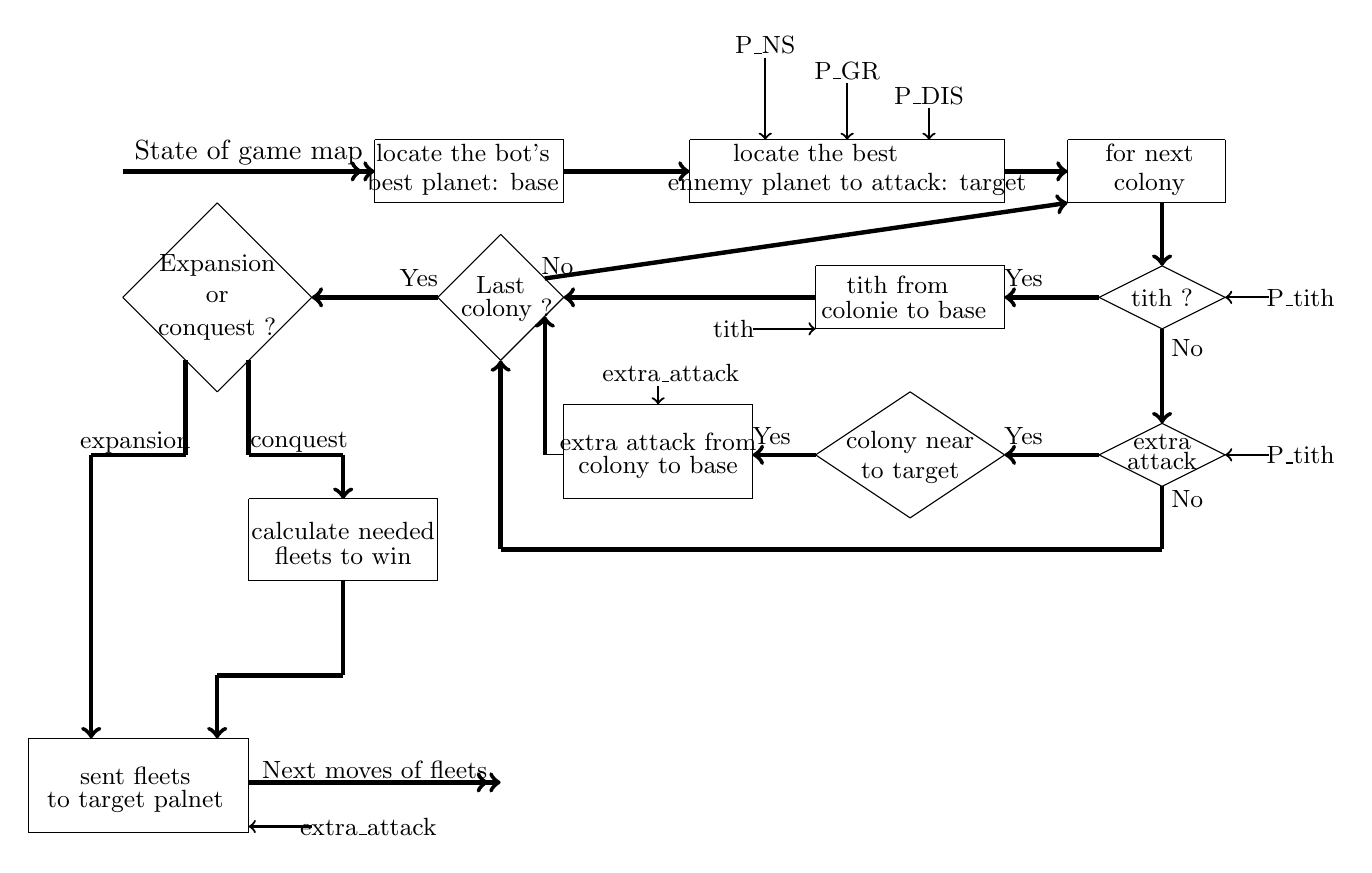
\begin{tikzpicture}[scale = 0.8]
\draw [->][ultra thick](-1,20) -- (3,20);
\draw [->][ultra thick](-1,20) -- (2.8,20);
\node at (1,20.3) {State of game map};
\draw (3,20.5) --(3,19.5);
\draw (3,20.5) --(6,20.5);
\draw (6,20.5) --(6,19.5);
\draw (6,19.5) --(3,19.5);
\draw [->][ultra thick](6,20) -- (8,20);
\node at (4.4,20.3) {\small locate the bot's};
\node at (4.4,19.8) {\small best planet: base};
\draw (8,20.5) --(8,19.5);
\draw (8,20.5) --(13,20.5);
\draw (13,20.5) --(13,19.5);
\draw (13,19.5) --(8,19.5);
\draw [->][thick](9.2,21.8) -- (9.2,20.5);
\draw [->][thick](10.5,21.4) -- (10.5,20.5);
\draw [->][thick](11.8,21) -- (11.8,20.5);
\node at (10,20.3) {\small locate the best};
\node at (9.2,22) {\small P\_NS};
\node at (10.5,21.6) {\small P\_GR};
\node at (11.8,21.2) {\small P\_DIS};
\node at (10.5,19.8) {\small ennemy planet to attack: target};
\draw [->][ultra thick](13,20) -- (14,20);
\draw (14,20.5) --(14,19.5);
\draw (14,20.5) --(16.5,20.5);
\draw (16.5,20.5) --(16.5,19.5);
\draw (16.5,19.5) --(14,19.5);
\node at (15.3,20.3) {\small for next};
\node at (15.3,19.8) {\small colony};
\draw [->][ultra thick](15.5,19.5) -- (15.5,18.5);
\draw (15.5,18.5) --(14.5,18);
\draw (14.5,18) --(15.5,17.5);
\draw (15.5,17.5) --(16.5,18);
\draw (16.5,18) --(15.5,18.5);
\draw [->][thick](17.2,18) -- (16.5,18);
\node at (17.7,18) {\small P\_tith};
\draw [->][thick](17.2,15.5) -- (16.5,15.5);
\node at (17.7,15.5) {\small P\_tith};
\node at (15.5,18) {\small tith ?};
\node at (15.5,15.7) {\small extra};
\node at (15.5,15.4) {\small attack};
\draw [->][ultra thick](15.5,17.5) -- (15.5,16);
\node at (15.9,17.2) {\small No};
\draw (15.5,16) --(14.5,15.5);
\draw (14.5,15.5) --(15.5,15);
\draw (15.5,15) --(16.5,15.5);
\draw (16.5,15.5) --(15.5,16);
\draw [->][ultra thick](14.5,18) -- (13,18);
\node at (13.3,18.3) {\small Yes};
\draw [ultra thick](15.5,15) -- (15.5,14);
\node at (15.9,14.8) {\small No};
\draw [ultra thick](15.5,14) -- (5,14);
\draw [->][ultra thick](5,14) -- (5,17);
\draw (13,18.5) --(13,17.5);
\draw (13,17.5) --(10,17.5);
\draw (10,17.5) --(10,18.5);
\draw (10,18.5) --(13,18.5);
\node at (13.3,15.8) {\small Yes};
\node at (11.3,18.2) {\small tith from};
\node at (11.4,17.8) {\small colonie to base};
\node at (8.7,17.5) {\small tith};
\draw [->][thick](9,17.5) -- (10,17.5);
\draw [->][ultra thick](14.5,15.5) -- (13,15.5);
\node at (9.3,15.8) {\small Yes};
\draw (13,15.5) --(11.5,16.5);
\draw (11.5,16.5) --(10,15.5);
\draw (10,15.5) --(11.5,14.5);
\draw (11.5,14.5) --(13,15.5);
\node at (11.5,15.7) {\small colony near};
\node at (11.5,15.2) {\small to target};
\draw [->][ultra thick](10,15.5) -- (9,15.5);
\draw (9,16.3) --(9,14.8);
\draw (9,14.8) --(6,14.8);
\draw (6,14.8) --(6,16.3);
\draw (6,16.3) --(9,16.3);
\node at (7.5,15.7) {\small extra attack from};
\node at (7.5,15.3) {\small colony to base};
\draw [->][thick](7.5,16.6) -- (7.5,16.3);
\node at (7.7,16.8) {\small extra\_attack};
\draw [->][ultra thick](10,18) -- (6,18);
\draw (6,18) --(5,19);
\draw (5,19) --(4,18);
\draw (4,18) --(5,17);
\draw (5,17) --(6,18);
\node at (5,18.2) {\small Last};
\node at (5.1,17.8) {\small colony ?};
\draw [->][ultra thick](5.7,18.3) -- (14,19.5);
\node at (5.9,18.5) {\small No};
\node at (3.7,18.3) {\small Yes};
\draw (6,15.5) -- (5.7,15.5);
\draw [->][ultra thick](5.7,15.5) -- (5.7,17.7);
\draw [->][ultra thick](4,18) -- (2,18);
\draw (2,18) -- (0.5,19.5);
\draw (0.5,19.5) -- (-1,18);
\draw (-1,18) -- (0.5,16.5);
\draw (0.5,16.5) -- (2,18);
\node at (0.5,18.5) {\small Expansion };
\node at (0.5,18) {\small or };
\node at (0.5,17.5) {\small conquest ?};
\draw [ultra thick](1,17) -- (1,15.5);
\draw [ultra thick](1,15.5) -- (2.5,15.5);
\node at (1.8,15.7) {\small conquest};
\draw [->][ultra thick](2.5,15.5) -- (2.5,14.8);
\draw (1,14.8) -- (4,14.8);
\draw (4,14.8) -- (4,13.5);
\draw (4,13.5) -- (1,13.5);
\draw (1,13.5) -- (1,14.8);
\node at (2.5,14.3) {\small calculate needed};
\node at (2.5,13.9) {\small fleets to win};
\draw [ultra thick](0,17) -- (0,15.5);
\draw [ultra thick](0,15.5) -- (-1.5,15.5);
\draw [->][ultra thick](-1.5,15.5) -- (-1.5,11);
\draw (-2.5,11) -- (1,11);
\draw (-2.5,9.5) -- (1,9.5);
\draw (-2.5,11) -- (-2.5,9.5);
\draw (1,11) -- (1,9.5);
\draw [ultra thick](2.5,13.5) -- (2.5,12);
\draw [ultra thick](2.5,12) -- (0.5,12);
\node at (-0.8,15.7) {\small expansion};
\draw [->][ultra thick](0.5,12) -- (0.5,11);
\node at (-0.8,10.4) {\small sent fleets};
\node at (-0.8,10) {\small to target palnet};
\draw [->][ultra thick](1,10.3) -- (4.8,10.3);
\draw [->][ultra thick](1,10.3) -- (5,10.3);
\node at (3,10.5) {\small Next moves of fleets};
\draw [->][thick](2,9.6) -- (1,9.6);
\node at (2.9,9.6) {\small extra\_attack};
\end{tikzpicture}
\caption{The states that are governing the behaviour of the AisBot including the parameters used on the evaluation of the bot's behaviour. these parameters will improve by the clonal selection algorithm (CLONALG).}
\end{figure*}

%%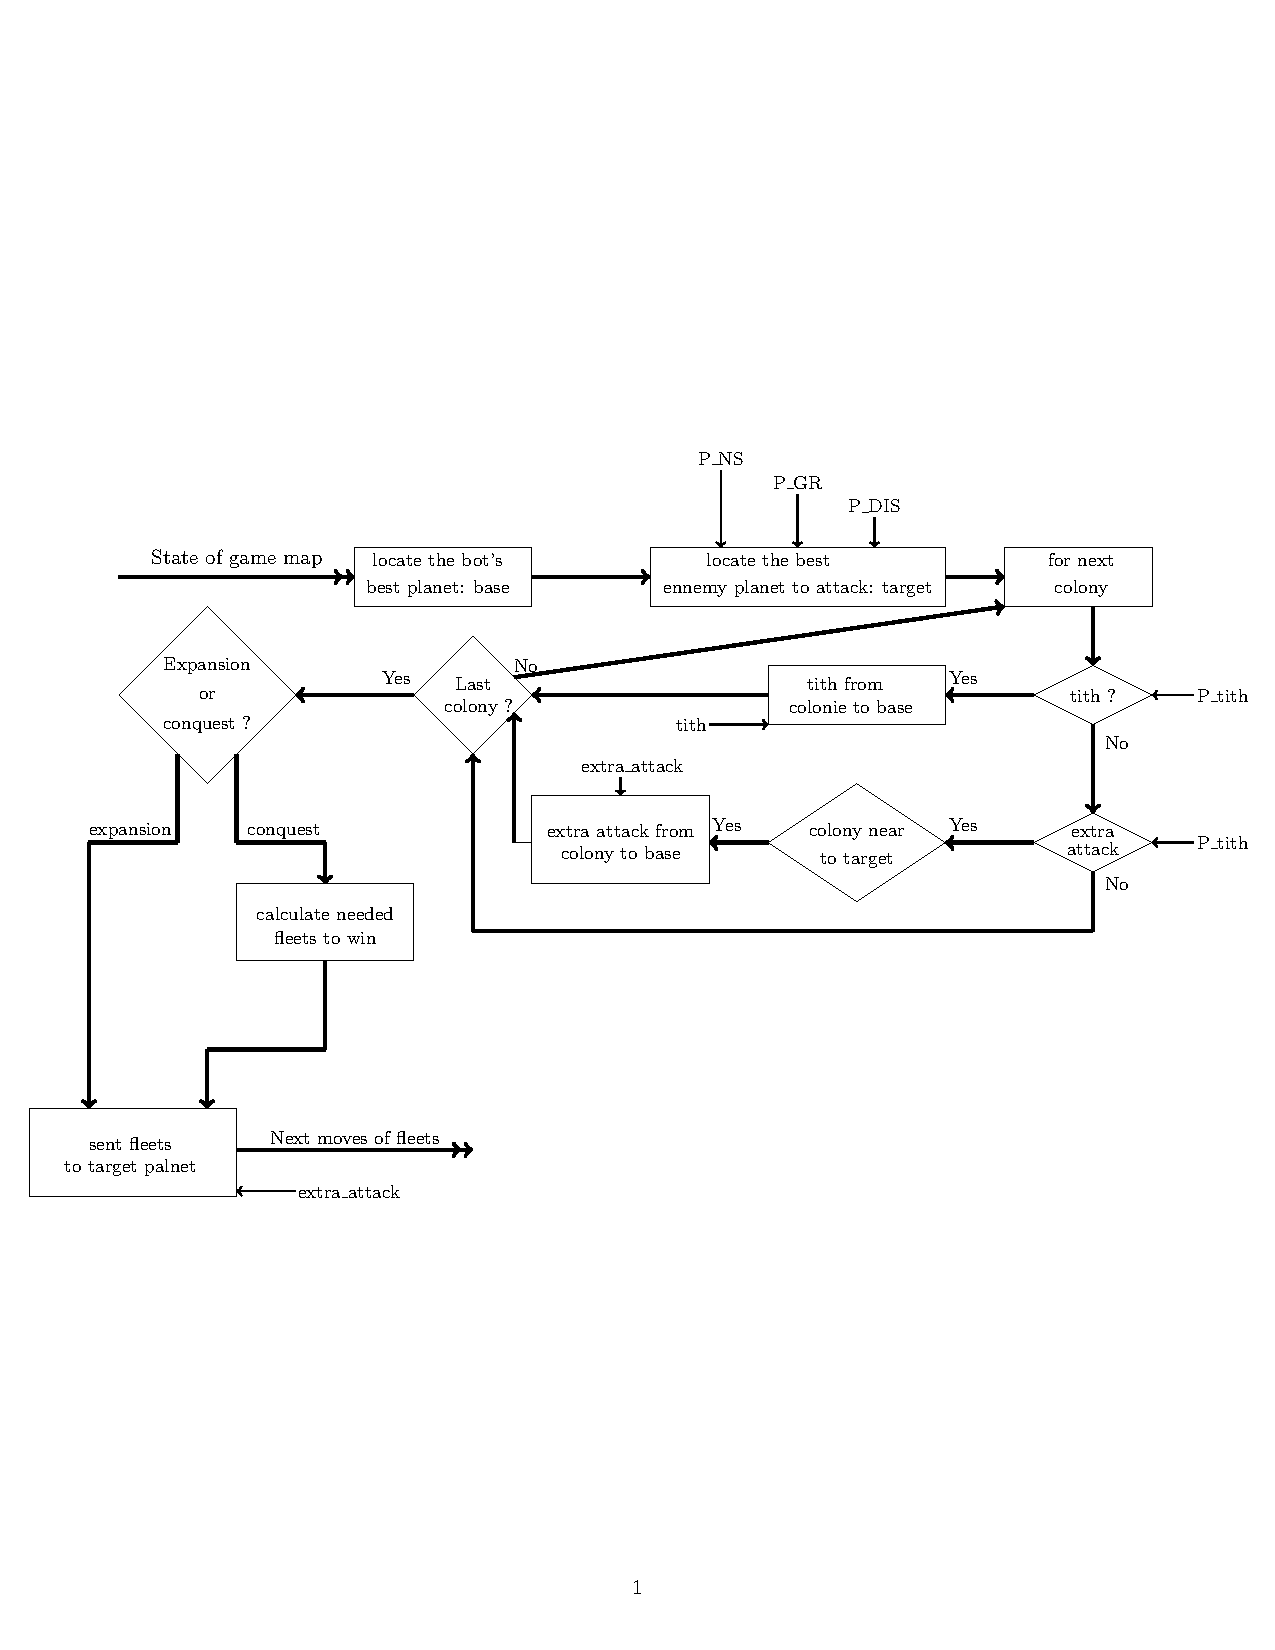
\includepdf[scale=0.7,pages=1]{botDiagram}


As we mentioned previously, the purpose of this study is to try to optimize the behaviour of a bot during the planet war RTS game. In order to improve our experimentation, we use the AisBot as a conquer bot in this game, and it works as follows: first of all, when a turn is started, the bot tries to determine the base planet based on a score function and the rest of planets are used as colonies.Secondly, the bot decides which planet to attack for the next turn or if it owns additional planet the action will be considered as a reinforcement, in order to reach the target planet, it can take some number of turns. If the bot trying to attack a target is owned by a neutral, the action will be considered as an expansion; however, if it's owned by the enemy, the action will be considered as a conquest. Once the base planet is reinforced by starships coming from colonies, the action will be considered as a Tith. In addition, when colonies that are closed to the target planet than the base is allowed to attack the target by sending fleets, instead of reinforcing the base and this one sends those fleets to the target planet, but move directly to the target. Besides, when a planet was targeted by the bot, it is no possible to decide another attack against the same planet until the first one finished, that is mean, for each fleet sent to perform an attack, it knows the target planet in its data structure. \\





In order to improve the behaviour of the bot,  a set of rules is defined included some parameters classified by weights, probabilities and amounts. the parameters signification is : 
\begin{itemize}
\item \textit{$Tith_{perc}$}: starships proportions that the bot can sends.
\item \textit{$Tith_{prob}$}: Tith probability that a colony sends to the base planet.
\item \textit{$w_{NS}$}: weight of starships number hosted on the planet.
\item \textit{$w_{DIS}$}: weight of distance between the base and the target planet.
\item \textit{$w_{GR}$}: weight of growth rate according to the target planet.
\item \textit{$Pool_{perc}$}: percentage of extra starships can send from the base to the target planet.
\item \textit{$Support_{perc}$}: Percentage of extra starships from the colony to the target.
\item \textit{$Support_{prob}$}: Probability of sending extra starships from the colony to the target.
\end{itemize}
Furthermore, each parameter takes some values during the optimization process depends on it meaning in the game, our conquer bot will be based on these values to make decisions during the game. To determine the target planet the bot will use a score function define as follow:

\begin{equation}
Score(p) = \frac{p.NumStarships.w_{NS-DIS}.Dist(base,p)}{1+p.GrowthRate.w_{GR}}
\end{equation}

Where the $w_{NS-dis}$ and the $w_{GR}$ are weights related successively to starships number, the growth rate for the planet and the distance to reach the target. As we mentioned above the $base$ is the planet which has the highest number of starships and $p$ refer to planet want to evaluate. \\ 

When the Tith and the attack process are performed by the colonies, the base planet also sends starships to attack the target. The number of starships sends to attack is estimated according to the attack mode, if the bot attack mode is expansion where the target does not generate starships during the game that implies the bot will integrate a very specific starships number to be able to defeat the planet target, in the other hand, if the bot attack mode is a conquest, the engine will estimate the number of troops needs to beat the enemy.




\subsection{RandomBot}
The development kit of google for the planet war game include an example of a bot called RandomBot, the behaviour of this bot is very simple and it works independently of any situation (map). based on it basic behaviour, the bot tries to send fleets randomly and try to perform random attacks without any estimation.If we compare the AisBot and the RandomBot behaviours, we will clearly find that the AisBot behaviour is more complex than the one on RandomBot, and it be able to defeat it in all situation and maps; however, it needs more turns to beat it; for this purpose, the greatest challenge is to make the AisBot's behaviour quite fast by determining the values of parameters shown in the previous section systematically.


\section{AisBot: an AIS optimization}
The aim of this optimization is to make the bot behave faster and be able to win in less number of turns, in order to do that, an artificial immune system (AIS) algorithm used on the set of rules included the parameters that will determine the behaviour of the bot; when the parameters are improved, they are fixed and will be uploaded by the bot in order to play a real scenario. \\
Therefore, the purpose is to determine the parameters values in order to evaluate the bot's behaviour.The AIS proposed in this study use a floating array to represent all parameters defined previously, while, the clonal proliferation process works on a totally new array with a specific proliferation factor for each parameter according to its fitness. The maturation mechanism is applied to the cloned antibodies by mutating the parameters values using the equation (1) with a probability amount to minimize the bad antibodies. \\

The selection process based on an evaluation technic by implementing tournaments where each cloned individual used to compete with the aim of being selected for the next generation from the best results were chosen. The evaluation of an individual is staged by including their parameters for the AisBot behaviour and placing the bot on a real planet war game against the RandomBot on five maps. \\

The aim of this optimization is to minimize the number of turns needs to win, the best bot is the one that plays fewer turns until win; this kind of ranking bots strongly shown a constraint problem is that each individual was able to win every single game.

\section{Exprementation and results}
With the aim of testing the CLONALG algorithm, the bot placed under several situations and play several games against the RandomBot. The algorithm parameters can be found on the Table 1:
\begin{table}[h!]
\centering
\begin{tabular}{ |c|c| }
\hline
 Number of antibodies & 20 \\ 
 Number of generations & 15 \\  
 maximun antbodies Cloned & 72 \\ 
 \hline   
\end{tabular}
\caption{Parameters used in the CLONALG algorithm}
\label{TABLE 1}
\end{table}


To make a bot under a real game scenario with optimized parameters will take hours, since, to evaluate each individual it took more seconds. The figure (4) showed the evaluation of the number of turns plays by the bot until win, and it appears that the number of turns needs to win in five maps decrease when the evaluation progress.Furthermore, in figure (5) two, the parameters evaluation is shown during the optimization process in amoung fifteen generations. \\

\begin{figure}
\begin{center}
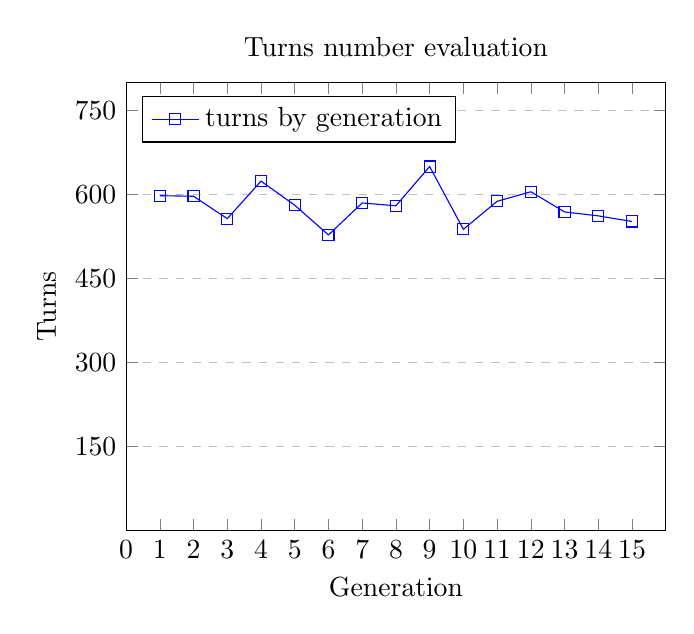
\begin{tikzpicture}
\begin{axis}[
    title={Turns number evaluation},
    xlabel={Generation},
    ylabel={Turns},
    xmin=0, xmax=16,
    ymin=0, ymax=800,
    xtick={0,1,2,3,4,5,6,7,8,9,10,11,12,13,14,15},
    ytick={150,300,450,600,750},
    legend pos=north west,
    ymajorgrids=true,
    grid style=dashed,
]
 
\addplot[
    color=blue,
    mark=square,
    ]
    coordinates {
    (1,598)(2,597)(3,557)(4,624)(5,581)(6,528)(7,585)(8,580)(9,650)(10,538)(11,588)(12,605)(13,569)(14,562)(15,552)
    };
    \legend{turns by generation}
 
\end{axis}
\end{tikzpicture}
\end{center}
\caption{the evaluation of the number of turns plays by the bot until win in 5 maps, and it appears that the number of turns needs to win in five maps decrease when the evaluation progress}
\end{figure}


\begin{figure}
\begin{center}
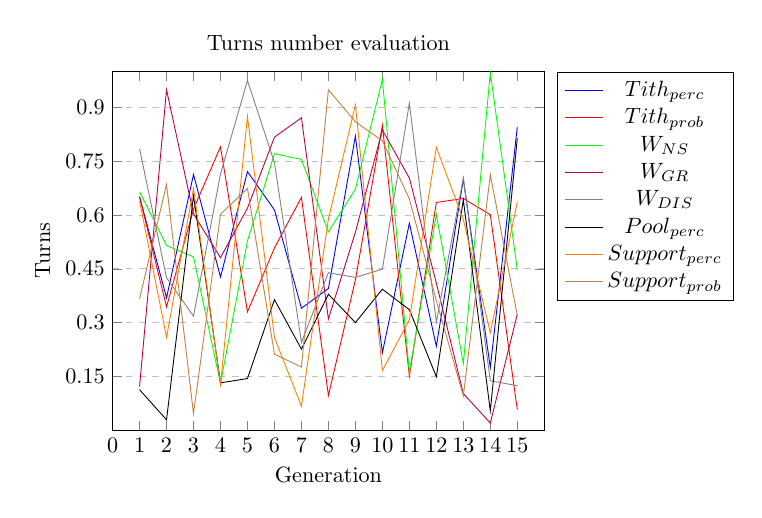
\begin{tikzpicture}[scale = 0.8]
\begin{axis}[
    title={Turns number evaluation},
    xlabel={Generation},
    ylabel={Turns},
    xmin=0, xmax=16,
    ymin=0, ymax=1,
    xtick={0,1,2,3,4,5,6,7,8,9,10,11,12,13,14,15},
    ytick={0.15,0.3,0.45,0.6,0.75,0.9},
    legend pos=outer north east,
    ymajorgrids=true,
    grid style=dashed,
]
 
\addplot[
    color=blue,
    ]
    coordinates{(1,0.651)(2,0.369)(3,0.713)(4,0.427)(5,0.721)(6,0.614)(7,0.34)(8,0.395)(9,0.82)(10,0.216)(11,0.577)(12,0.234)(13,0.7)(14,0.175)(15,0.845)};
    
    \addplot[
    color=red,
    ]
    coordinates{(1,0.651)(2,0.344)(3,0.616)(4,0.79)(5,0.33)(6,0.508)(7,0.649)(8,0.097)(9,0.419)(10,0.85)(11,0.151)(12,0.635)(13,0.646)(14,0.601)(15,0.057)};
    
    \addplot[
    color=green,
    ]
    coordinates{(1,0.665)(2,0.515)(3,0.483)(4,0.13)(5,0.528)(6,0.771)(7,0.755)(8,0.553)(9,0.672)(10,0.978)(11,0.161)(12,0.602)(13,0.186)(14,0.997)(15,0.447)};
    
    \addplot[
    color=purple,
    ]
    coordinates{(1,0.122)(2,0.949)(3,0.603)(4,0.481)(5,0.619)(6,0.817)(7,0.871)(8,0.31)(9,0.552)(10,0.837)(11,0.703)(12,0.41)(13,0.102)(14,0.02)(15,0.323)};
    
    \addplot[
    color=gray,
    ]
    coordinates{(1,0.785)(2,0.425)(3,0.318)(4,0.714)(5,0.975)(6,0.746)(7,0.245)(8,0.439)(9,0.426)(10,0.449)(11,0.912)(12,0.301)(13,0.703)(14,0.138)(15,0.124)};
    
    \addplot[
    color=black,
    ]
    coordinates{(1,0.113)(2,0.029)(3,0.654)(4,0.132)(5,0.144)(6,0.364)(7,0.226)(8,0.379)(9,0.3)(10,0.393)(11,0.336)(12,0.149)(13,0.642)(14,0.054)(15,0.814)};
    
    \addplot[
    color=orange,
    ]
    coordinates{(1,0.64)(2,0.259)(3,0.674)(4,0.127)(5,0.875)(6,0.258)(7,0.067)(8,0.589)(9,0.907)(10,0.166)(11,0.308)(12,0.789)(13,0.587)(14,0.272)(15,0.636)};
    
    \addplot[
    color=brown,
    ]
    coordinates{(1,0.366)(2,0.685)(3,0.046)(4,0.602)(5,0.674)(6,0.212)(7,0.176)(8,0.949)(9,0.86)(10,0.807)(11,0.645)(12,0.361)(13,0.096)(14,0.712)(15,0.32)};
    
    
    \legend{$Tith_{perc}$,$Tith_{prob}$,$W_{NS}$,
    $W_{GR}$,$W_{DIS}$,$Pool_{perc}$,$Support_{perc}$,$Support_{prob}$}
 
\end{axis}
\end{tikzpicture}
\end{center}
\caption{the evaluation of the Parameters during the optimization process}
\end{figure}



Table II describes the evaluated results improved by the optimization process where the colonies have a high probability to send Tith to the base (0.84) by sending a fewer hosted starships which can be explained that the colonies have to deserve there starships to defend it-selves in an emergency. On the other hand, the probability for a planet to perform an attack against other ones is around (0.32) and the proportion of sending troops is elevated (64\%) when there is an attack action. Based on this, when a planet performs an attack, the base also can send a high extra starships number for the attack around 81\%. Finally, when the bot trying to determine the target planet to perform the attack, the most important weights based on is the number of starships hosted on the target and the growth rate related to it, the distance has a less priority in this process. \\

\begin{table*}
\centering
\begin{tabular}{|c|c|c|c|c|c|c|c|c|}
\hline
 & $Tith_perc$ & $Tith_prob$ & $W_NS$ & $W_GR$ & $W_DIS$ & $Pool_perc$ & $Support_perc$ & $Support_prob$ \\ 
 \hline
 Before & 0.959 & 0.651 & 0.665 & 0.122 & 0.785 & 0.113 & 0.64 & 0.366 \\  
 \hline
 After & 0.057 & 0.845 & 0.447 & 0.323 & 0.124 & 0.814 & 0.636 & 0.32 \\
 \hline  
\end{tabular}
\caption{Parameters used in the CLONALG algorithm}
\label{TABLE 2}
\end{table*}

\begin{table*}
\centering
\begin{tabular}{|c|c|c|c|c|c|}
\hline
 Maps & 5 & 10 & 20 & 50 & 100 \\ 
 \hline
 Before & 135 & 128 & 161 & 102 & 144 \\  
 \hline
 After & 98 & 80 & 70 & 72 & 87 \\
 \hline  
\end{tabular}
\caption{results after 5 games of our AisBot with random parameters and after the optimization against the RandomBot}
\label{TABLE 3}
\end{table*}

In general, the optimised AisBot is able to defeat the RandomBot in all situations with a minimum number of turns, this can demonstrate that the application of an Evolutionary Algorithm reach some hight capabilities in optimization behaviour even a parametrize behaviour as the one used on the AisBot. There are a lot of challenges can explore all the capabilities of AIS algorithms in the design of the bot's behaviour can offer.


\section{conclusions}
The planet wars game it was classified as an RTS game, where the player (bots) fight against others in real-time. The main aim of this study is to investigate the application of the Evolutionary Algorithms (EAs) and the better results can be obtained in real-world problems, by tunning real game scenarios that used a parametrise behaviour of a bot tuning by an AIS Algorithm. This problem showed that the EAs can improve the evaluation of a hand-coded bot by defeating multiple opponents in different situations in fewer turns. In the other hand, the high capabilities of an evolutionary approach can be improved at least in this type of problems.

%\subsubsection{Subsubsection Heading Here}
%Subsubsection text here.


% An example of a floating figure using the graphicx package.
% Note that \label must occur AFTER (or within) \caption.
% For figures, \caption should occur after the \includegraphics.
% Note that IEEEtran v1.7 and later has special internal code that
% is designed to preserve the operation of \label within \caption
% even when the captionsoff option is in effect. However, because
% of issues like this, it may be the safest practice to put all your
% \label just after \caption rather than within \caption{}.
%
% Reminder: the "draftcls" or "draftclsnofoot", not "draft", class
% option should be used if it is desired that the figures are to be
% displayed while in draft mode.
%
%\begin{figure}[!t]
%\centering
%\includegraphics[width=2.5in]{myfigure}
% where an .eps filename suffix will be assumed under latex, 
% and a .pdf suffix will be assumed for pdflatex; or what has been declared
% via \DeclareGraphicsExtensions.
%\caption{Simulation results for the network.}
%\label{fig_sim}
%\end{figure}

% Note that the IEEE typically puts floats only at the top, even when this
% results in a large percentage of a column being occupied by floats.


% An example of a double column floating figure using two subfigures.
% (The subfig.sty package must be loaded for this to work.)
% The subfigure \label commands are set within each subfloat command,
% and the \label for the overall figure must come after \caption.
% \hfil is used as a separator to get equal spacing.
% Watch out that the combined width of all the subfigures on a 
% line do not exceed the text width or a line break will occur.
%
%\begin{figure*}[!t]
%\centering
%\subfloat[Case I]{\includegraphics[width=2.5in]{box}%
%\label{fig_first_case}}
%\hfil
%\subfloat[Case II]{\includegraphics[width=2.5in]{box}%
%\label{fig_second_case}}
%\caption{Simulation results for the network.}
%\label{fig_sim}
%\end{figure*}
%
% Note that often IEEE papers with subfigures do not employ subfigure
% captions (using the optional argument to \subfloat[]), but instead will
% reference/describe all of them (a), (b), etc., within the main caption.
% Be aware that for subfig.sty to generate the (a), (b), etc., subfigure
% labels, the optional argument to \subfloat must be present. If a
% subcaption is not desired, just leave its contents blank,
% e.g., \subfloat[].


% An example of a floating table. Note that, for IEEE style tables, the
% \caption command should come BEFORE the table and, given that table
% captions serve much like titles, are usually capitalized except for words
% such as a, an, and, as, at, but, by, for, in, nor, of, on, or, the, to
% and up, which are usually not capitalized unless they are the first or
% last word of the caption. Table text will default to \footnotesize as
% the IEEE normally uses this smaller font for tables.
% The \label must come after \caption as always.
%
%\begin{table}[!t]
%% increase table row spacing, adjust to taste
%\renewcommand{\arraystretch}{1.3}
% if using array.sty, it might be a good idea to tweak the value of
% \extrarowheight as needed to properly center the text within the cells
%\caption{An Example of a Table}
%\label{table_example}
%\centering
%% Some packages, such as MDW tools, offer better commands for making tables
%% than the plain LaTeX2e tabular which is used here.
%\begin{tabular}{|c||c|}
%\hline
%One & Two\\
%\hline
%Three & Four\\
%\hline
%\end{tabular}
%\end{table}


% Note that the IEEE does not put floats in the very first column
% - or typically anywhere on the first page for that matter. Also,
% in-text middle ("here") positioning is typically not used, but it
% is allowed and encouraged for Computer Society conferences (but
% not Computer Society journals). Most IEEE journals/conferences use
% top floats exclusively. 
% Note that, LaTeX2e, unlike IEEE journals/conferences, places
% footnotes above bottom floats. This can be corrected via the
% \fnbelowfloat command of the stfloats package.




%\section{Conclusion}
%The conclusion goes here.




% conference papers do not normally have an appendix


% use section* for acknowledgment
%\section*{Acknowledgment}


%The authors would like to thank...





% trigger a \newpage just before the given reference
% number - used to balance the columns on the last page
% adjust value as needed - may need to be readjusted if
% the document is modified later
%\IEEEtriggeratref{8}
% The "triggered" command can be changed if desired:
%\IEEEtriggercmd{\enlargethispage{-5in}}

% references section

% can use a bibliography generated by BibTeX as a .bbl file
% BibTeX documentation can be easily obtained at:
% http://mirror.ctan.org/biblio/bibtex/contrib/doc/
% The IEEEtran BibTeX style support page is at:
% http://www.michaelshell.org/tex/ieeetran/bibtex/
%\bibliographystyle{IEEEtran}
% argument is your BibTeX string definitions and bibliography database(s)
\bibliography{references}

\addcontentsline{toc}{section}{Bibliography}

\bibliographystyle{abbrv}
%
% <OR> manually copy in the resultant .bbl file
% set second argument of \begin to the number of references
% (used to reserve space for the reference number labels box)
%\begin{thebibliography}{1}

%\bibitem{IEEEhowto:kopka}
%H.~Kopka and P.~W. Daly, \emph{A Guide to \LaTeX}, 3rd~ed.%\hskip 1em plus
 % 0.5em minus 0.4em\relax Harlow, England: Addison-Wesley, 1999.

%\end{thebibliography}




% that's all folks
\end{document}


